\section{Resultados}

\newread\tmp

\openin\tmp=../exp/shopping.s.entropy
\read\tmp to \ShoppingSEntropy
\closein\tmp

\openin\tmp=../exp/shopping.s1.entropy
\read\tmp to \ShoppingSOneEntropy
\closein\tmp

\openin\tmp=../exp/starbucks.s.entropy
\read\tmp to \StarbucksSEntropy
\closein\tmp

\openin\tmp=../exp/starbucks.s1.entropy
\read\tmp to \StarbucksSOneEntropy
\closein\tmp

\openin\tmp=../exp/wired_lan.s.entropy
\read\tmp to \WiredLanSEntropy
\closein\tmp

\openin\tmp=../exp/wired_lan.s1.entropy
\read\tmp to \WiredLanSOneEntropy
\closein\tmp

\subsection{Escenario 1 (Red cableada)}

\begin{tikzpicture}[baseline]
    \begin{axis}[
            title={},
            xlabel={Símbolo (Destino)},
            ylabel={Cantidad de información},
            scaled x ticks=false,
            scaled y ticks=false,
            width=0.45\textwidth,
            height=0.35\textwidth,
            bar width=2cm,
            ymin=0,
            enlarge x limits=0.65,
            xtick=data,
            major tick length=0,
            xticklabels={$s_{\texttt{UNICAST}}$, $s_{\texttt{BROADCAST}}$},
            x tick label style={rotate=80,anchor=east,font=\small},
            legend entries={$H(\mathcal{S})$,$H_{\max}(\mathcal{S})$},
            legend style={
                legend cell align=left,
                legend pos=north east
            }
        ]
        \addplot[
                ybar,
                fill=blue!10,
                draw=blue,
                forget plot
            ] table[x=IsBroadcast,y=Information]{../exp/wired_lan.s.information};
        \addplot[mark=none, blue, thick, update limits=false] {\WiredLanSEntropy};
        \addplot[mark=none, blue, thick, dashed, update limits=false] {1};
    \end{axis}
\end{tikzpicture}

\begin{tikzpicture}[baseline]
    \begin{axis}[
            title={},
            xlabel={Símbolo (Dirección IP)},
            ylabel={Cantidad de información},
            scaled x ticks=false,
            scaled y ticks=false,
            width=0.45\textwidth,
            height=0.35\textwidth,
            legend pos=outer north east,
            legend cell align=left,
            ymin=0,
            xtick=data,
            xticklabels from table={../exp/wired_lan.s1.information}{IP},
            x tick label style={rotate=80,anchor=east,font=\small}
        ]
        \addplot [
                ybar,
                fill=blue!10,
                draw=blue,
                select coords between index={0}{20}
            ] table[x=X-Pos,y=Information]{../exp/wired_lan.s1.information};

        \coordinate (A) at (axis cs:0,\WiredLanSOneEntropy);
        \coordinate (O1) at (rel axis cs:0,0);
        \coordinate (O2) at (rel axis cs:1,0);

        \draw [blue, thick] (A -| O1) -- (A -| O2);

    \end{axis}
\end{tikzpicture}

\begin{figure}[H]
    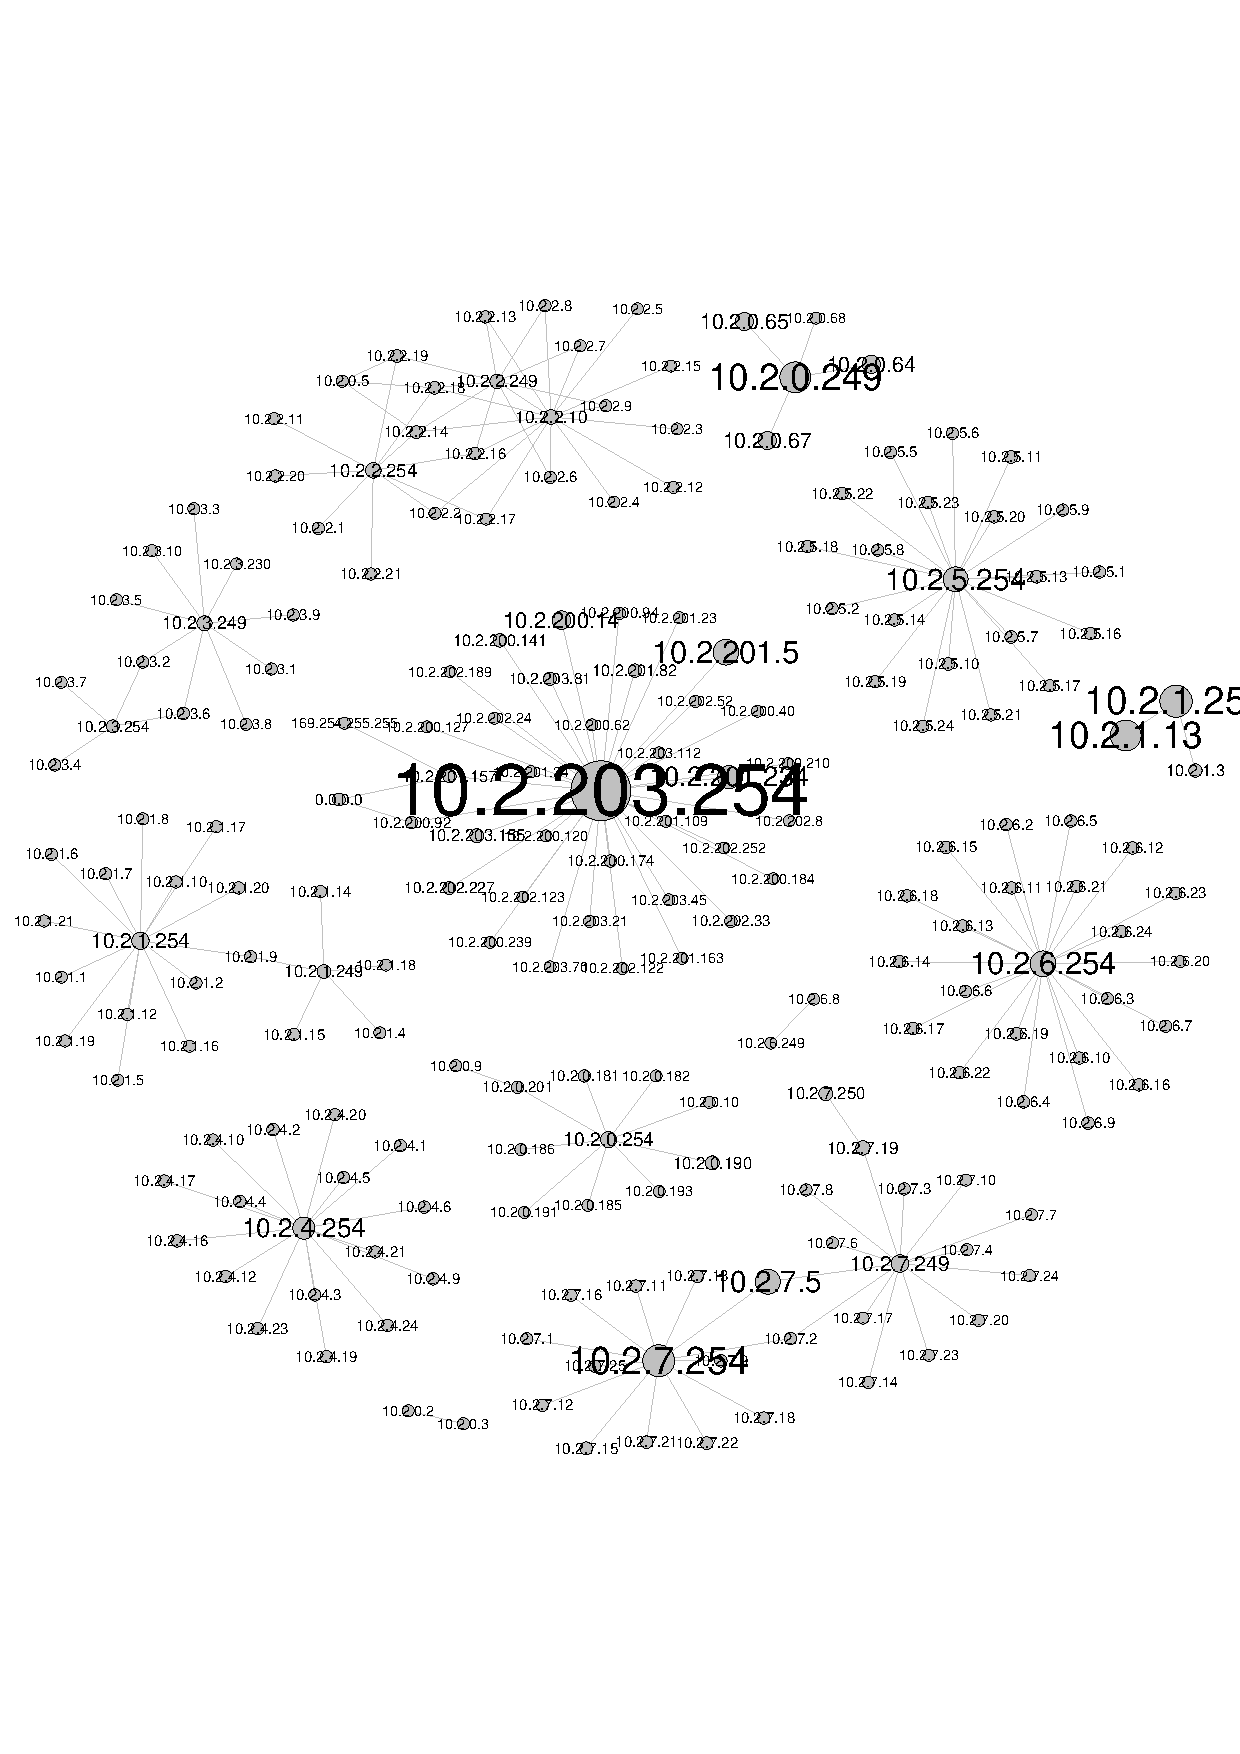
\includegraphics[scale=0.4]{figures/wired_lan.pdf}
    \caption{Red de mensajes \texttt{ARP} para captura de red cableada.}
\end{figure}

\subsection{Escenario 2 (\emph{Shopping})}

\begin{tikzpicture}[baseline]
    \begin{axis}[
            title={},
            xlabel={Símbolo (Destino)},
            ylabel={Cantidad de información},
            scaled x ticks=false,
            scaled y ticks=false,
            width=0.45\textwidth,
            height=0.35\textwidth,
            bar width=2cm,
            ymin=0,
            enlarge x limits=0.65,
            xtick=data,
            major tick length=0,
            xticklabels={$s_{\texttt{UNICAST}}$, $s_{\texttt{BROADCAST}}$},
            x tick label style={rotate=80,anchor=east,font=\small},
            legend entries={$H(\mathcal{S})$,$H_{\max}(\mathcal{S})$},
            legend style={
                legend cell align=left,
                legend pos=north west
            }
        ]
        \addplot[
                ybar,
                fill=blue!10,
                draw=blue,
                forget plot
            ] table[x=IsBroadcast,y=Information]{../exp/shopping.s.information};
        \addplot[mark=none, blue, thick, update limits=false] {\ShoppingSEntropy};
        \addplot[mark=none, blue, thick, dashed, update limits=false] {1};
    \end{axis}
\end{tikzpicture}

\begin{tikzpicture}[baseline]
    \begin{axis}[
            title={},
            xlabel={Símbolo (Dirección IP)},
            ylabel={Cantidad de información},
            scaled x ticks=false,
            scaled y ticks=false,
            width=0.45\textwidth,
            height=0.35\textwidth,
            legend pos=outer north east,
            legend cell align=left,
            ymin=0,
            xtick=data,
            xticklabels from table={../exp/shopping.s1.information}{IP},
            x tick label style={rotate=80,anchor=east,font=\small}
        ]
        \addplot[
                ybar,
                fill=blue!10,
                draw=blue,
                select coords between index={0}{20}
            ] table[x=X-Pos,y=Information]{../exp/shopping.s1.information};

        \coordinate (A) at (axis cs:0,\ShoppingSOneEntropy);
        \coordinate (O1) at (rel axis cs:0,0);
        \coordinate (O2) at (rel axis cs:1,0);

        \draw [blue, thick] (A -| O1) -- (A -| O2);

    \end{axis}
\end{tikzpicture}

\begin{figure}[H]
    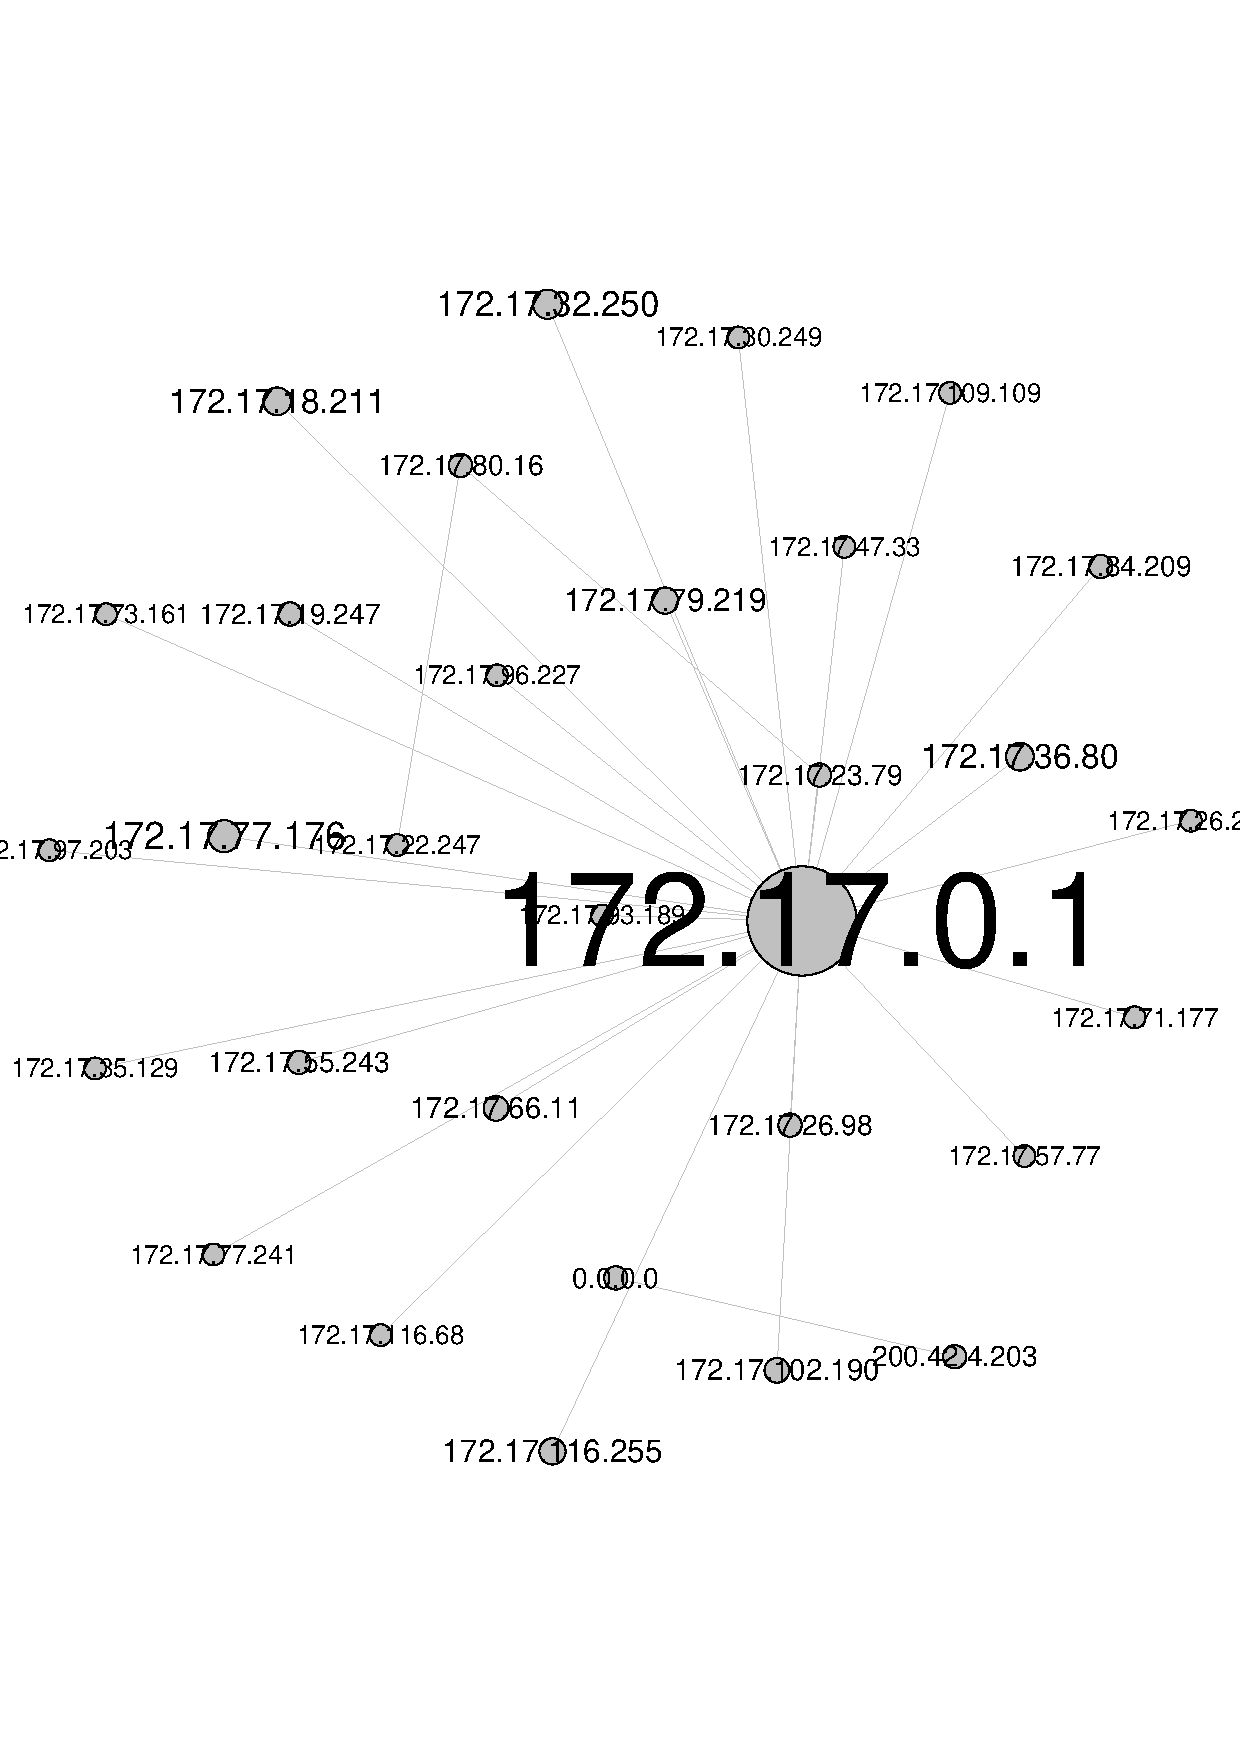
\includegraphics[scale=0.4]{figures/shopping.pdf}
    \caption{Red de mensajes \texttt{ARP} para captura del shopping.}
\end{figure}

\subsection{Escenario 3 (\emph{Starbucks})}

\begin{tikzpicture}[baseline]
    \begin{axis}[
            title={},
            xlabel={Símbolo (Destino)},
            ylabel={Cantidad de información},
            scaled x ticks=false,
            scaled y ticks=false,
            width=0.45\textwidth,
            height=0.35\textwidth,
            bar width=2cm,
            ymin=0,
            enlarge x limits=0.65,
            xtick=data,
            major tick length=0,
            xticklabels={$s_{\texttt{UNICAST}}$, $s_{\texttt{BROADCAST}}$},
            x tick label style={rotate=80,anchor=east,font=\small},
            legend entries={$H(\mathcal{S})$,$H_{\max}(\mathcal{S})$},
            legend style={
                legend cell align=left,
                legend pos=north west
            }
        ]
        \addplot[
                ybar,
                fill=blue!10,
                draw=blue,
                forget plot
            ] table[x=IsBroadcast,y=Information]{../exp/starbucks.s.information};
        \addplot[mark=none, blue, thick, update limits=false] {\StarbucksSEntropy};
        \addplot[mark=none, blue, thick, dashed, update limits=false] {1};
    \end{axis}
\end{tikzpicture}

\begin{tikzpicture}[baseline]
    \begin{axis}[
            title={},
            xlabel={Símbolo (Dirección IP)},
            ylabel={Cantidad de información},
            scaled x ticks=false,
            scaled y ticks=false,
            width=0.45\textwidth,
            height=0.35\textwidth,
            legend pos=outer north east,
            legend cell align=left,
            ymin=0,
            xtick=data,
            xticklabels from table={../exp/starbucks.s1.information}{IP},
            x tick label style={rotate=80,anchor=east,font=\small}
        ]
        \addplot [ybar, fill=blue!10, draw=blue] table[x=X-Pos,y=Information]
                {../exp/starbucks.s1.information};

        \coordinate (A) at (axis cs:0,\StarbucksSOneEntropy);
        \coordinate (O1) at (rel axis cs:0,0);
        \coordinate (O2) at (rel axis cs:1,0);

        \draw [blue, thick] (A -| O1) -- (A -| O2);

    \end{axis}
\end{tikzpicture}

\begin{figure}[H]
    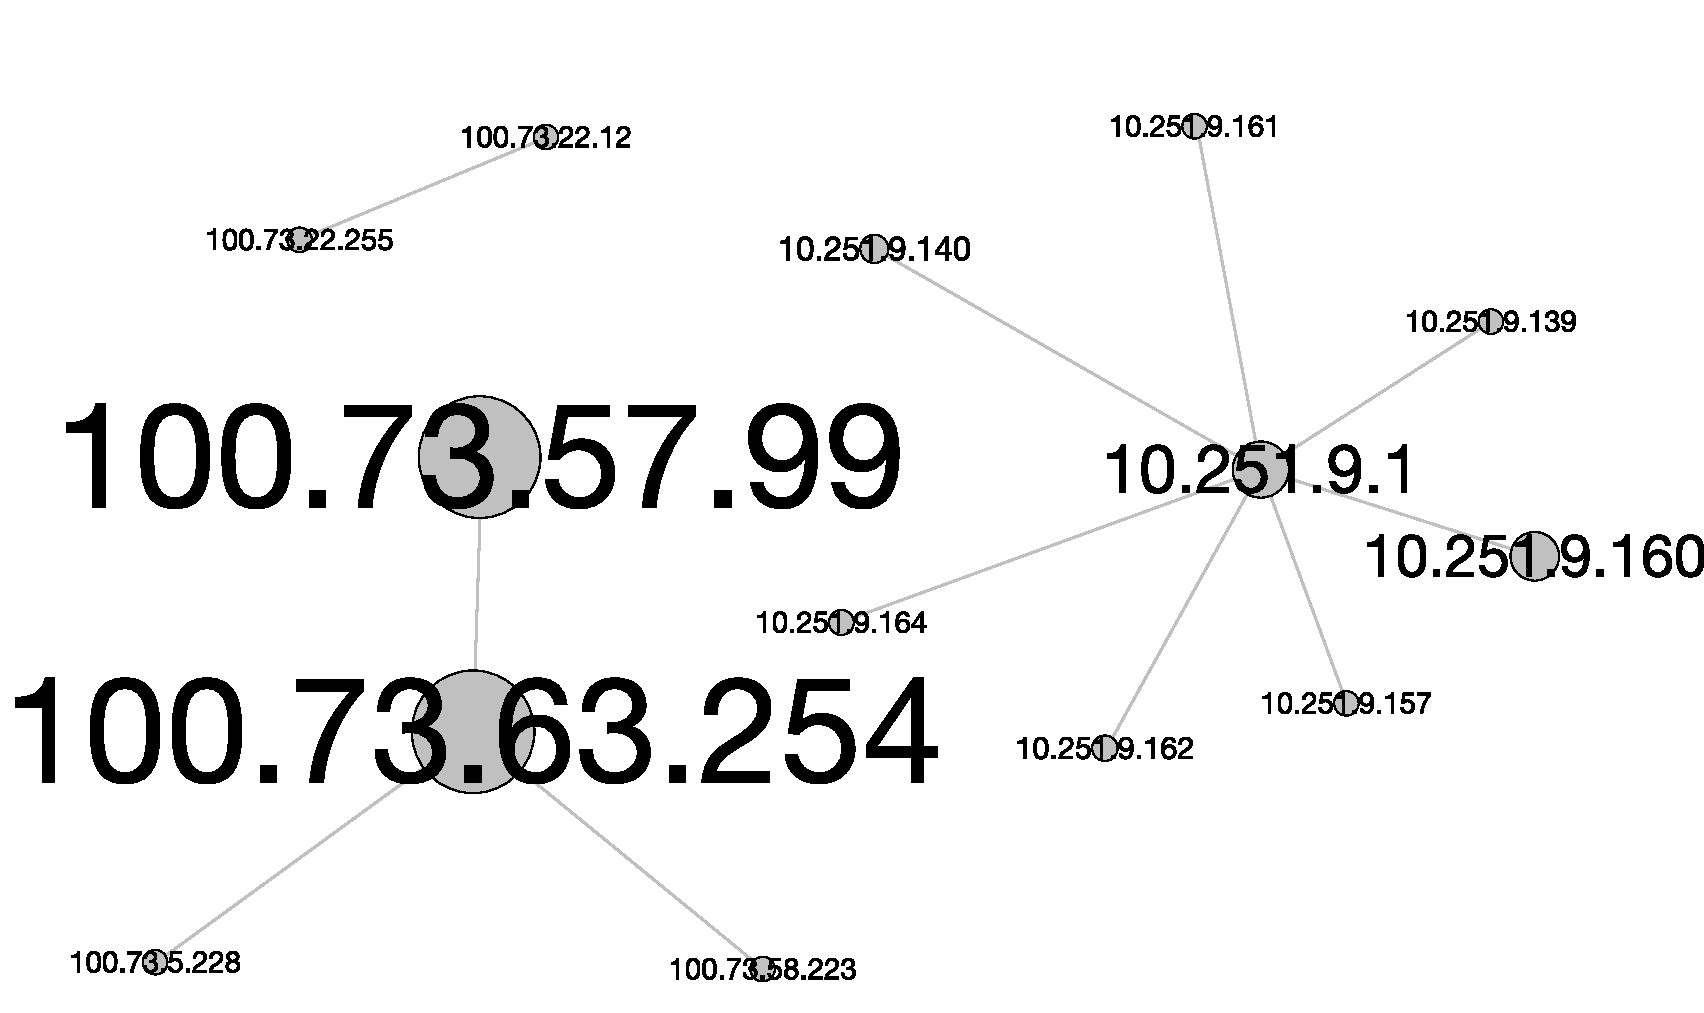
\includegraphics[scale=0.4]{figures/starbucks.pdf}
    \caption{Red de mensajes \texttt{ARP} para captura del Starbucks.}
\end{figure}
